\normalfont\normalsize
\chapter{Software Environment: Contiki Operating System}

software intro ....


The software is composed on diferent interlocking (trebuie modificat ) modules running on diferent devices and operating systems.

The modules are written mainly in java and c.

again ... andrei ?

\begin{figure}[ht]
\begin{center}
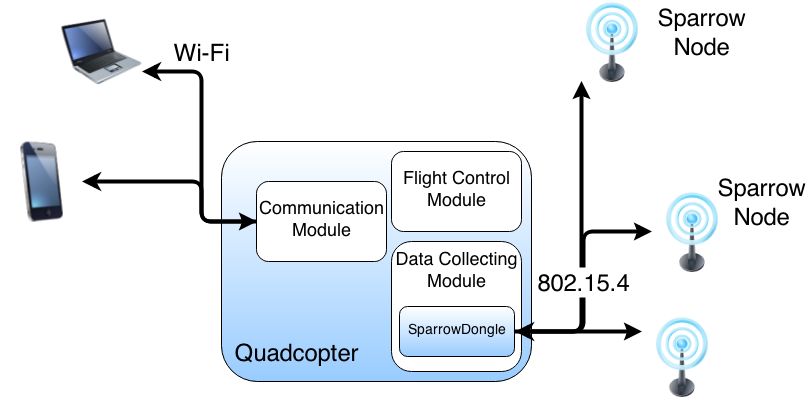
\includegraphics[width=0.9\textwidth]{sw_platform/organigrama.png}
\end{center}
\caption{\small \itshape{Modules and connections between them and devices}}
\end{figure}


\clearpage

\section{The Data Collecting Module}

The module saves the collected data int-o the drones internal memory and prases the data in order to obtain certain informations like number of nodes currently connected to the dongle, de signal strength etc. This informations are passed to the communication module to provide to the user realtime feedback.

The memory area in which the informations sent to the user are saved is shared between this module and the comunication module. Basically, the way this two modules interract with each other can be compared to the consumer - producer problem, where the Data Collecting Module can be associated with the producer side and the Communication Module with the consumer side.

The main problem consists of deadlocks and data starvation. This is prevent with the use of one mutex that allows only one thread at a time to moddify the informations.

\lstset{numbers=none, mathescape=true, nolol=false,caption=Data Collection use of mutex,label=lst:task}
\begin{lstlisting}
pthread_mutex_lock(&data_lock); 
add_node_data(get_current_timestamp(),read_data + 7);
pthread_mutex_unlock(&data_lock);
\end{lstlisting}

The mutex is used similarly in the Communication Module when it consumes the information.

\lstset{numbers=none, mathescape=true, nolol=false,caption=Data Collection use of mutex,label=lst:task}
\begin{lstlisting}
void add_node_data(long long time_stamp , char *p) {
	int i;
	int id = get_hex(p,2);

	/* the power of the signal calculated in dB */	
	int power = -90 + 3* (get_hex(p + 64,2)-1);


	/* creating a file with unique name */
	char file_name[100];
	sprintf(file_name, "/node_logs/%lli_%i",file_timestamp,id);
	/* opening a file in append mode */	
	FILE *fptr = fopen(file_name,"a");
	
	/* saving the new data at the end of the file */
	fprintf(fptr,"%s",p);
	fclose(fptr);
	
	/* searching for previous connection of the same node*/
	for(i = 0 ;i < node_nr;i++) {
		if(data[i].id == id) {
			/* timestamp update - node is stil reachable and sending data */
			data[i].time_stamp = time_stamp;
			return;
		}
	}

	/* new node found by the drone */
	data[node_nr].id = id;
	data[node_nr].time_stamp = time_stamp;
	node_nr ++;
}

\end{lstlisting}


\clearpage

\section{The Communication Module}


\clearpage

\section{The Saved Data Transfer Module}
